% !Mode:: "TeX:UTF-8"
\documentclass[13pt]{ctexbeamer}


\usepackage{amsmath,amssymb,amsthm}             % AMS Math
\usepackage{graphicx}
\usepackage{epstopdf}
\usepackage{tikz}
\linespread{1.3}

\usepackage{mathrsfs}  %花写字母
 

%%%=== theme ===%%%
% \usetheme{Warsaw}
%\usetheme{Copenhagen}
%\usetheme{Singapore}
\usetheme{Madrid}
%\usefonttheme{professionalfonts}
%\usefonttheme{serif}
% \usefonttheme{structureitalicserif}
%%\useinnertheme{rounded}
%%\useinnertheme{inmargin}
\useinnertheme{circles}
%\useoutertheme{miniframes}
\setbeamertemplate{navigation symbols}{}
%\setbeamertemplate{footline}[page number]
\setbeamertemplate{footline}[frame number] 


%\usepackage[fontset=mac]{ctex}
%\usepackage{ctex}


\usepackage{hyperref}
\usepackage{tipa}

\titlegraphic{
\includegraphics[width=2cm]{tjnu.jpg}} 

\setbeamertemplate{theorems}[numbered]
\newtheorem{thm}{定理}
\newtheorem{lem}{引理}
\newtheorem{exa}{例}
\newtheorem*{theo}{定理}
\newtheorem*{conj}{猜想}
\newtheorem*{defi}{定义}
\newtheorem*{coro}{推论}
\newtheorem*{ex}{练习}
\newtheorem*{rem}{注}
\newtheorem*{prop}{性质}
\newtheorem*{qst}{问题}

\def\qed{\nopagebreak\hfill{\rule{4pt}{7pt}}\medbreak}
\def\pf{{\bf 证明~~ }}
\def\sol{{\bf 解~~ }}



\def\R{\mathbb{R}}
\def\Rn{\mathbb{R}^n}
\def\A{\mathscr{A}}
\def\B{\mathscr{B}}
\def\D{\mathscr{D}}
\def\E{\mathscr{E}}
\def\O{\mathscr{O}}

\def\rank{\operatorname{rank}}
\def\dim{\operatorname{dim}}
\def\0{\mathbf{0}}
\def\a{\alpha}
\def\b{\beta}
\def\r{\gamma}

\usepackage{color}
\definecolor{linkcol}{rgb}{0,0,0.4}
\definecolor{citecol}{rgb}{0.5,0,0}

\definecolor{blue}{rgb}{0,0.08,1}
\newcommand{\blue}{\textcolor{blue}}

  \usepackage{graphicx}
  \DeclareGraphicsExtensions{.eps}
%   \usepackage[a4paper,pagebackref,hyperindex=true,pdfnewwindow=true]{hyperref}


\begin{document}



\title[让LaTeX跑起来]{论文写作指导  ---  让LaTeX跑起来}
\author[]{{\large 张彪} }
\institute[]{{\normalsize
		天津师范大学\\[6pt]
		zhang@tjnu.edu.cn}}

\date{}


%
%\AtBeginSection[]
%{
%\begin{frame}
%	\frametitle{Outline}
%	\tableofcontents[currentsection]
%\end{frame}
%\setcounter{exa}{0}
%\setcounter{equation}{0}
%}



\begin{frame}
\maketitle
\end{frame}


\begin{frame}
	\frametitle{\textcolor{orange}{Outline}}
	\tableofcontents
\end{frame}




\section{LaTeX}

\subsection{LaTex 简介}
\begin{frame}
	\begin{itemize}
	\item 	TeX
($\backslash$t\textepsilon x$\backslash$,常被读作$\backslash$t\textepsilon k$\backslash$,音译“泰赫”,“泰克”,写作“TEX”)

\item 它在学术界特别是数学、物理学和计算机科学界十分流行。
	\item
TeX被普遍认为是一个优秀的排版工具,尤其是对于复杂数学公式的处理。
	\item
利用LaTeX等终端软件,TeX就能够排版出精美的文本以帮助人们辨认和查找。
\end{itemize}
\end{frame}


\begin{frame}{TeX}
	
	
	\begin{columns}[c]  %开始进入分栏环境,居中设置
		
		\column{6cm}
		
		\begin{itemize}
			\item
			TeX
			是一个由美国计算机教授高德纳(Donald Ervin Knuth)编写的排版软件。
			
			\item 高德纳最早开始自行编写TeX的原因,是因为当时的电脑排版技术十分粗糙,已经影响到他的巨著《计算机程序设计艺术》的印刷质量。作为一名计算机学家,他决定自行编写一个排版软件:TeX。
		\end{itemize}
		
		
		%\rightline{ {\Large 一华罗庚 \qquad \qquad\qquad}}
		\column{5cm} 
		\begin{figure}[p]
			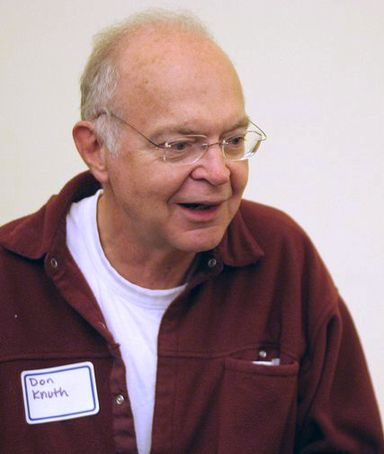
\includegraphics[scale=0.5]{Knuth.jpg}
			\caption{Donald Knuth(1938-~~)}
		\end{figure}
		
	\end{columns}
	
	
\end{frame}


\begin{frame}{LaTeX}
	\begin{columns}[c]  %开始进入分栏环境,居中设置
		
		\column{6cm}
		
\begin{itemize}
	\item LaTeX,是一种基于TEX的排版系统,由美国计算机科学家Leslie~ Lamport~(2013年获图灵奖)在20世纪80年代初期开发。
	\item 利用这种格式系统的处理,即使用户没有排版和程序设计的知识也可以充分发挥由TEX所提供的强大功能,不必一一亲自去设计或校对,能在几天,甚至几小时内生成很多具有书籍质量的印刷品。
\end{itemize}
		
	
		\column{5cm} 
		\begin{figure}[p]
			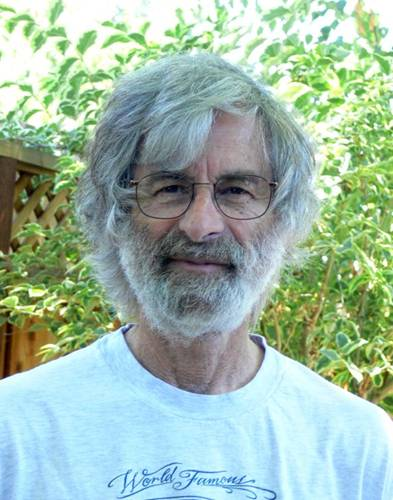
\includegraphics[scale=0.4]{Lamport.jpg}
			\caption{Lamport(1941-~~)}
		\end{figure}
		
	\end{columns}


\end{frame}


\begin{frame}{LaTeX}

\begin{itemize}
\item     LaTeX 是 基于 TeX 的排版系统。
    
\item 实际上 LaTeX 利用 TeX 的控制命令,定义了许多新的控制命令并封装成一个可执行文件。
    
\item这个可执行文件会去解释 LaTeX 新定义的命令成为 TeX 的控制命令,并最终交由 TeX 引擎进行排版。

\item LaTeX 实际上是一个工具,它将用户按照它的格式编写的文档解释成 TeX 引擎能理解的形式并交付给 TeX 引擎处理,再将最终结果返回给用户。
\end{itemize}

    
    
 
\end{frame}



\begin{frame}{LaTeX}
\begin{itemize}
	\item 对于生成复杂表格和数学公式,这一点表现得尤为突出。因此它非常适用于生成高印刷质量的科技和数学、物理文档。这个系统同样适用于生成从简单的信件到完整书籍的所有其他种类的文档。
	\item LaTeX使用TeX作为它的格式化引擎,当前的版本是LaTeX2e(写作“LATEX2ε”)。
\end{itemize}
\end{frame}

\begin{frame}{LaTeX 发音和书写}
	\begin{itemize}
\item 	由于TEX一词应该读作“泰赫”($\backslash$t\textepsilon x$\backslash$),所以LATEX一词可以音译为“拉泰赫”。
\item 
	在英语中,IATEX实际通常读作
$\backslash$le\i t\textepsilon k$\backslash$
(音译“莱泰克”)或者(音译“拉泰克”)
$\backslash$l\textscripta\textlengthmark t\textepsilon k$\backslash$
\item 
	LATEX的开发者Lamport表示对LATEX的读音没有偏好。
		\end{itemize}
	\vspace{15pt}
		\begin{itemize}
\item 
LaTeX的正确的写法是
\begin{center}

\includegraphics[scale=0.08]{LATEX.jpg}
\end{center}
如果因技术限制而无法做到,则应该写成“LaTeX”。
\item 
不得改变任何一个字母的大小写,以免和“latex” (乳胶) 混淆。
	\end{itemize}

	
	

	
	

\end{frame}
\subsection{中文排版}


\begin{frame}{中文排版}
\begin{itemize}
    \item 高德纳教授在实现 TeX 的当初并没有考虑到中日韩等字符的处理,而只支持 ASCII 字符。
    \item 在 XeTeX 出现之前,为了能让 TeX 系统排版中文,国人曾使用了 天元、CCT、CJK 等手段处理中文。其中 天元和 CCT 现在已经基本不用,CJK 因为使用时间长且效果相对较好,现在还有人使用。

    \end{itemize}
\end{frame}
    
    
    
    
\begin{frame}{CTeX 中文套装}


\begin{itemize}
	\item 
	CTeX 中文套装是中国科学院吴凌云研究员开发的一种中文LaTeX排版系统,他在MiKTeX的基础上增加了对中文的完整支持。
	\item 
	网站  http://www.ctex.org/
%	\item CTeX 套装是科学院吴凌云研究员的个人作品。

\item CTeX 中文套装集成了WinEdt, SumatraPDF等工具软件。
\end{itemize}
在 CTeX 套装刚刚问世之时,因其解决了中文的排版问题,所以广受欢迎。 但是,
\begin{itemize}
	\item  一方面 CTeX 套装已经很久不更新(最新的稳定版本	v2.9.2.164 -- 2012.03.22),内里的宏包、工具陈旧;
	\item 另一方面,XeLaTeX等技术逐渐成熟,可以更简便地完成中文排版;
\end{itemize}

	因此,\alert{现在不推荐使用 CTeX 中文套装}。

%不要安装和使用 CTeX 套装!
%如\documentclass{ctexart}
\end{frame}

    
\begin{frame}{XeTeX}

\begin{itemize}
    \item 不同于 CJK 等方式使用 TeX 和 pdfTeX 这两个不直接支持 Unicode 字符的引擎,\alert{XeTeX 引擎}直接支持 Unicode 字符。也就是说现在不使用 CJK 也能排版中日韩文的文档了,并且这种方式要比之前的方式更加优秀。
    
    \item XeLaTeX 和 XeTeX 的关系与 pdfLaTeX 和 pdfTeX 的关系类似,这里不再赘述。

 \item  使用 XeTeX 引擎需要使用 \alert{UTF-8 编码}。{UTF-8 编码}是 Unicode 编码的一种。
\end{itemize}
\end{frame}




\begin{frame}
{CTeX 宏集}
\begin{itemize}
	\item 
虽然它的名字也是「CTeX」,但是 CTeX 宏集和 CTeX 套装是两个不同的东西。
\item  CTEX 宏集支持LATEX、pdfLATEX、XƎLATEX、LuaLATEX、upLATEX 等多种不同的编译方式,并为它们提供了统一的界面。主要功能由宏包ctex 以及中文文档类ctexart、ctexrep、ctexbook 和 ctexbeamer 实现。
\item 我们推荐\alert{优先使用 CTeX 宏集处理中文}。
\item 中文的文档可以直接使用ctex 文档类。
%也就是ctexart、ctexrep、ctexbook、ctexbeamer 这些。
\end{itemize}

 
%请在任何情况下优先使用 CTeX 宏集在 LaTeX 中处理中文!
\end{frame}

\subsection{LaTeX发行版与编辑器}
\begin{frame}{LaTeX发行版}
\begin{itemize}
	\item MiKTex 
		\begin{itemize}
	\item
	MiKTeX 是 mick-tech 公司 TEX/LATEX 最新的
实施方案及相关程序 MiKTEX 集成软件包
管理器可以从互联网中安装缺失的部分宏
包。
\end{itemize}
	\item CTeX中文套装 (基于MiKTeX,支持中文,已停更)
	
	\item \alert{TeX Live} 
	\begin{itemize}
	\item
	TeX Live是由国际TeX用户组(TUG)整理和发布的TeX软件发行套装,包含与TeX系统相关的各种程序、编辑与查看工具、常用宏包及文档、常用字体及多国语言支持。
		\item
	TeX Live是许多Linux/Unix系统默认或推荐的TeX套装,同时也支持包括Windows和Mac OS X等在内的其它操作系统。
	\end{itemize}

	\item MacTeX -- macOS(OS X)系统下的一个定
制化的 TeXLive 版本。

\item proTeXt -- MiKTeX-based distribution for Windows 
\end{itemize}
\end{frame}


\begin{frame}{TeX Live}

\begin{itemize}
	\item TeX Live 是 TUG (TeX User Group) 维护和发布的 TeX 系统,可说是「官方」的 TeX 系统。
	\item 我们推荐任何阶段的 TeX 用户,都尽可能使用 TeX Live,以保持在跨操作系统平台、跨用户的一致性。
	\item TeX Live 的官方站点是 \href{https://tug.org/texlive/}{https://tug.org/texlive/}
	\item 建议尝试使用国内大学的镜像站下载。
	
	\href{https://mirrors.ustc.edu.cn/CTAN/systems/texlive/Images/} {https://mirrors.ustc.edu.cn/CTAN/systems/texlive/Images/}
	
	
	\href{https://mirrors.tuna.tsinghua.edu.cn/CTAN/systems/texlive/Images/}{https://mirrors.tuna.tsinghua.edu.cn/CTAN/systems/texlive/Images/}
	
\end{itemize}
\end{frame} 


\begin{frame}{编辑器}
\begin{itemize}
\item  TeXStudio (推荐使用)
\item TeXmaker
\item TeXworks (TexLive自带)
\item TexPad (for Mac users)
\item WinEdt
\end{itemize}
\end{frame}



\begin{frame}{推荐使用TeXLive + TeXStudio }
	推荐安装最新版本的
	
	\begin{itemize}
		\item TeXLive 
		
		\href{https://www.tug.org/texlive/}{https://www.tug.org/texlive/}
		
		
		
		\item TeXStudio
		
		http://www.texstudio.org/
	\end{itemize}
	
	TeXLive + TeXStudio  ~安装指南,可以参考
	\begin{itemize}
		\item 	\href{https://zhuanlan.zhihu.com/p/80603542}{https://zhuanlan.zhihu.com/p/80603542}
		\item \href{https://blog.csdn.net/yeler082/article/details/80665186}{https://blog.csdn.net/yeler082/article/details/80665186}
	\end{itemize}
\end{frame}



\begin{frame}{线上Latex:  Overleaf}
网站 
\href{https://www.overleaf.com/
}{https://www.overleaf.com/
}
\begin{itemize}
\item 在线编辑

\item 免安装,免配置

\item 多人协作

\item 版本管理
\end{itemize}
\end{frame}


\begin{frame}{Latex模板}
\begin{itemize}
    \item Latex工作室  
    \href{https://www.latexstudio.net/}{https://www.latexstudio.net/}
    \item Overleaf 
    \href{https://www.overleaf.com/
}{https://www.overleaf.com/
}
\end{itemize}
    
\end{frame}

\section{Mathpix Snip - 数学公式识别神器}
\begin{frame}{Mathpix Snip}
\begin{itemize}
	\item 截图识别公式,一键转换成 LaTeX 代码。
	
\href{https://mathpix.com/}{https://mathpix.com/}
\end{itemize}
\end{frame} 


\section{Tables Generator - 表格识别神器 }
\begin{frame}{Tables Generator }
\begin{itemize}
	\item 	 像在 Excel 里一样使用表格,一键转换成 LaTeX 代码。 
	\href{ http://www.tablesgenerator.com/}{ http://www.tablesgenerator.com/}

\end{itemize}


\end{frame}


\section{JabRef-文献管理软件}
\begin{frame}{JabRef}
\begin{itemize}
\item  JabRef

\href{https://www.jabref.org/}{https://www.jabref.org/}
\end{itemize}
\end{frame} 
\end{document} 